\documentclass[pdf]{beamer}
\mode<presentation>{\usetheme{Warsaw}}
\usepackage[T1,T2A]{fontenc}         % внутрішнє кодування шрифтів (може бути декілька);
                                          % вказане останнім діє по замовчуванню;
                                          % кириличне має співпадати з заданим в ukrhyph.tex.
\usepackage[utf8]{inputenc}       % кодування документа; замість cp866nav
                                          % може бути cp1251, koi8-u, macukr, iso88595, utf8.
\usepackage[english,ukrainian]{babel} % національна локалізація; може бути декілька
\usepackage{mystyle}

\newcommand{\red}[1]{{\color[rgb]{0.6,0,0}#1}}

\title{Поездка в Китай на 2 недели}
\subtitle{Пекин (7дн.), Шанхай(1д.), Санья(5д.), Гонконг(1д.)}
\setbeamertemplate{background canvas}{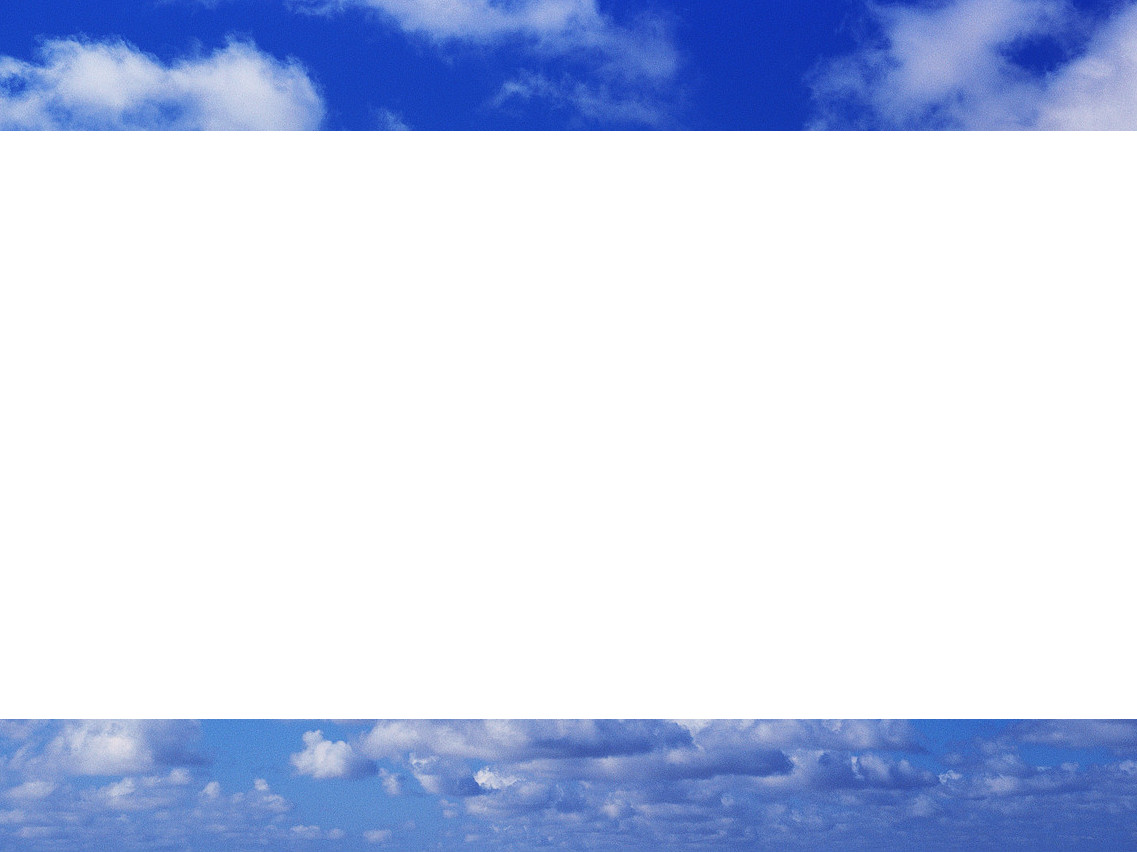
\includegraphics[width=\paperwidth,height=\paperheight]{clouds.jpg}}

\begin{document}
\begin{frame}\titlepage\end{frame}
	\begin{frame}{Пекин -- Площадь Tianmen}
		\mypic{0.8}{travel_china/tianmen.jpg}
		 Самая большая городская площадь в мире (440 кв. км.). Если правильно помню, там по вечерам многие любят запускать
		 воздушных змеев.
	\end{frame}
	\begin{frame}{Пекин -- Запретный город}
		\mypic{0.8}{travel_china/forbidden.jpg}
		 Самый обширный дворцовый комплекс в мире, главный дворцовый комплекс китайских императоров с XV по начало XX века. 
		 Только император и его приближенные имели право здесь находиться, а для простых смертных эта часть Пекина
		 была недоступна (отсюда название).
	\end{frame}
\end{document}
